\chapter{Architecture Generale et Choix Techniques} \label{chap:archgenerale}
\minitoc
\clearpage


\section{Introduction}

La création d’une distribution Linux personnalisée implique des décisions techniques et conceptuelles rigoureuses afin de garantir la \textbf{compatibilité} du système avec le matériel et les logiciels existants.  \\

Dans ce chapitre, nous allons  présenter : Architecture Générale de notre système, architecture cible  et   à quel ensemble de standards   nous appartenons.

 


\section{Architecture générale de la distribution Linux}
Avant de détailler chaque composant, il est essentiel de décrire le cadre général du système et de préciser les architectures matérielles que nous visons.

\begin{figure}[htbp]
    \centering
    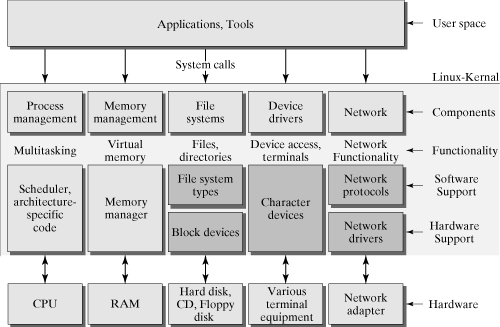
\includegraphics[width=1\textwidth]{images_pfe/linuxarchi.png}
    \caption{Couches de l’architecture d’un système Linux}
    \label{fig:linux-archi}
\end{figure}

Comme le montre la figure, un système se compose de trois couches principales :

\begin{enumerate}
  \item \textbf{Couche matérielle} : regroupe tous les périphériques physiques (RAM, disque dur, processeur, etc.).
  \item \textbf{Noyau} : composant central du système d’exploitation, il interagit directement avec le matériel et fournit des services bas niveau aux couches supérieures. \textcolor{blue}{(Nous en discuterons en détail au chapitre \ref{subsec:noyau-modules}}.)
  \item \textbf{Espace utilisateur} :  
    \begin{itemize}
      \item \textbf{Shell} : interface avec le noyau, masquant sa complexité et transmettant les commandes de l’utilisateur aux \textbf{appels système}.
      \item \textbf{Utilitaires} : programmes fournissant la majeure partie des fonctionnalités offertes à l’utilisateur.
    \end{itemize}
\end{enumerate}

Pour bien cadrer notre distribution, deux questions doivent guider nos choix :

\begin{enumerate}[label=\arabic*)]
  \item Quelles architectures matérielles cibles souhaitons-nous supporter ?
 % \item Quel noyau  allons-nous utiliser ?
  \item Quels standards  devons-nous utiliser pour assurer la portabilité et la compatibilité ?
\end{enumerate}

\section{Architectures physique cibles}
\label{subsec:arch-cibles}

. Le choix des architectures cibles conditionne en effet les outils de compilation, les optimisations et les bibliothèques à intégrer.

\begin{table}[htbp]
  \centering
  \caption{Types d’architectures de processeur (exemple)}
  \label{tab:architectures}
  \begin{tabular}{|l| l| c| l|}
    \toprule
    \textbf{Architecture} & \textbf{Type} & \textbf{Largeur (bits)} & \textbf{Cas d'utilisation} \\
    \midrule
    x86-64   & CISC & 64           & Stations de travail, serveurs \\ \hline
    ARM64    & RISC & 64           & Mobile, embarqué, serveurs    \\ \hline
    MISP    & RISC   &  32 / 64      & Routeurs, systèmes embarqués, usage éducatif \\ \hline
    RISC-V   & RISC & 32/64/128    & Usage académique, matériel sur mesure \\\hline
    POWER    & RISC & 64           & Serveurs d'entreprise, calcul haute performance \\
    \bottomrule
  \end{tabular}
\end{table}

Dans notre distribution , nous avons choisi comme architectures cibles  les processeurs \textbf{AMD et Intel x86\_64 }, en raison de leur compatibilité étendue et de leur support matériel mature. 


%\section{Pourquoi choisir le noyau Linux plutôt que le noyau Windows ?}

%\subsection*{1. Architecture}
%Le noyau Windows est souvent décrit comme un noyau hybride, combinant des éléments de micro- et de noyau monolithique : un microcœur gère les fonctions de %base, tandis que des composants comme les pilotes et systèmes de fichiers s’exécutent en mode noyau.  
%Le noyau Linux est principalement monolithique : tous les services nécessaires (pilotes, systèmes de fichiers, etc.) sont intégrés dans un bloc unique de %code s’exécutant en mode noyau.

%La distinction entre mode utilisateur et mode noyau existe dans les deux cas, mais Windows sépare strictement applications et opérations noyau, alors que %Linux expose davantage de fonctionnalités et de flexibilité dans le noyau lui-même.

%\subsection*{2. Philosophie de conception}
%\begin{itemize}
 % \item \textbf{Windows} : noyau propriétaire développé par Microsoft ; personnalisation et transparence limitées.  
 % \item \textbf{Linux} : noyau open source, modifiable et redistribuable librement.  
  %  Il supporte les modules noyau dynamiques, pouvant être chargés ou déchargés à chaud, offrant une grande flexibilité et facilitant mises à jour et %personnalisations.
%\end{itemize}

%\subsection*{3. Gestion des processus}
%Les deux noyaux assurent une isolation forte des processus, mais Linux offre un contrôle plus granulaire de l’ordonnancement et de l’allocation des %ressources (cgroups, nice, etc.).

%\subsection*{4. Gestion de la mémoire virtuelle}
%\begin{itemize}
%  \item \textbf{Windows} : mémoire virtuelle complexe avec fichier d’échange (pagefile) et compression en mémoire.  
%  \item \textbf{Linux} : pagination à la demande et mécanismes de cache agressifs, souvent plus performants. De nombreux outils (Valgrind, perf) facilitent le suivi et la détection de fuites de mémoire.
%\end{itemize}

%\subsection*{5. Pilotes de périphériques}
%\begin{itemize}
 % \item \textbf{Windows} : modèle de pilote spécifique, large prise en charge matérielle, mais signature Microsoft requise pour la sécurité.  
  %\item \textbf{Linux} : chargement dynamique des pilotes en modules, simplifiant l’ajout de nouveaux matériels sans redémarrage.
%\end{itemize}

%\subsection*{6. Appels système et API}
%\begin{itemize}
 % \item \textbf{Windows} : API riche (WinAPI) étroitement liée au noyau.  
  %\item \textbf{Linux} : ensemble d’appels système standardisés, utilisé par les applications pour invoquer les services du noyau.
%\end{itemize}

%\bigskip
%\noindent
%\textbf{En résumé}, le noyau Linux nous offre :
%\begin{itemize}
 % \item Un contrôle total du code source pour une personnalisation extrême,  
 % \item Une gestion fine de la mémoire et des ressources,  
 % \item Un pilotage précis des appels système,  
 % \item La capacité de charger et décharger immédiatement des pilotes matériels via les modules, sans redémarrage.
%\end{itemize}


\section{Normes de notre distibution}
\label{subsec:standards}

La structure de du systeme  respecte  les standards Linux suivants :

\begin{itemize}
  \item \textbf{POSIX}  
  \item \textbf{FHS } 
  \item \textbf{LSB  }
\end{itemize}


\subsection{POSIX}
\label{sssec:posix}
La norme POSIX (Interface portable pour systèmes d'exploitation) a été conçue pour standardiser un ensemble de fonctionnalités essentielles qu’un système d'exploitation doit fournir. Elle spécifie notamment une interface de programmation, un shell de commande ainsi qu’un ensemble d'outils classiques, dans le but de rendre les logiciels facilement transférables entre différentes plateformes de type Unix. 

\paragraph{Pourquoi POSIX est‑il important ?}
\begin{enumerate}
  \item Assurer la \textbf{portabilité} des logiciels entre systèmes de type UNIX (Linux, macOS, BSD, etc.).
  \item Fournir une API cohérente pour les appels système, la gestion des fichiers et le pilotage des processus.
  \item Aider les développeurs à écrire des applications \textbf{cross‑platform} sans réécrire leur code pour chaque OS.
\end{enumerate}


\textcolor{blue}{Pour plus d’informations sur POSIX, consultez \cite{posix}}

\subsection{Filesystem Hierarchy Standard (FHS) }
\label{sssec:fhs}
Le standard FHS (Filesystem Hierarchy Standard) définit une organisation logique des fichiers et répertoires dans les systèmes de type UNIX. Son objectif est d’assurer une cohérence dans la structure du système, facilitant ainsi la compatibilité des logiciels, des outils d’administration et des scripts. Il permet également de maintenir une documentation structurée et homogène entre différentes distributions Linux 



La structure de \textsc{Kraken OS} suit scrupuleusement ce standard (voir figure\textcolor{blue}{~\ref{fig:fsl}}).

\begin{figure}[H]
  \centering
  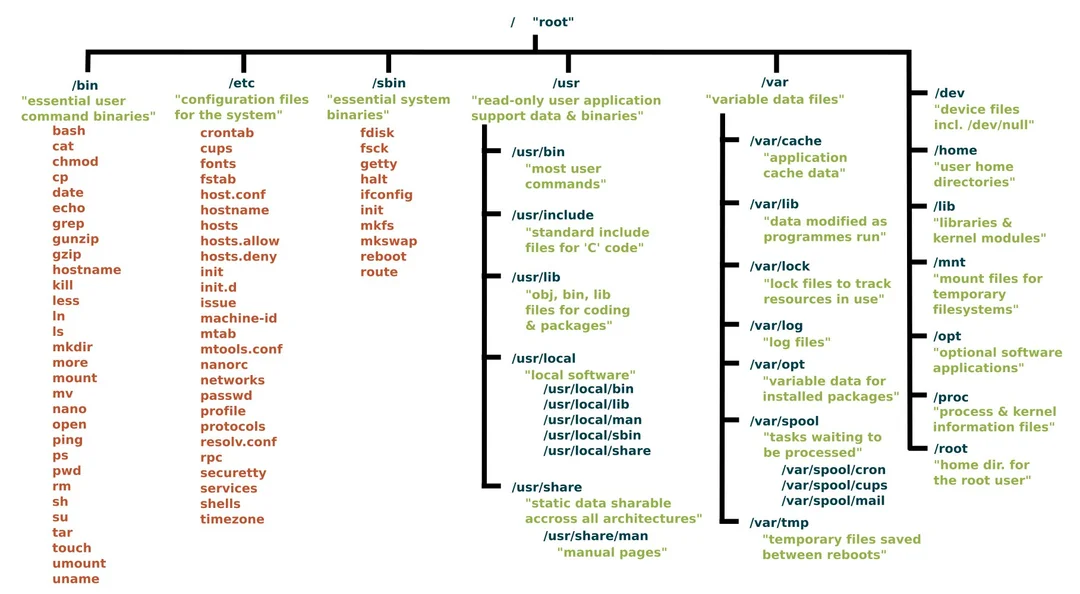
\includegraphics[width=0.85\textwidth]{images_pfe/fslinux.png}
  \caption{Architecture du système de fichiers conforme au standard FHS }
  \label{fig:fsl}
\end{figure}




Les principaux répertoires comprennent :

\begin{itemize}
    \item \textbf{Répertoires essentiels} :
    \begin{itemize}
        \item \texttt{/bin}, \texttt{/sbin} : Liens symboliques vers \texttt{/usr/bin} et \texttt{/usr/sbin} (conformément aux bonnes pratiques de sécurité)
        \item \texttt{/lib}, \texttt{/lib64} : Liens vers \texttt{/usr/lib} et \texttt{/usr/lib64} (centralisation des bibliothèques)
    \end{itemize}
    
    \item \textbf{Répertoires systèmes critiques} :
    \begin{itemize}
        \item \texttt{/etc} : Configuration système globale (fichiers \texttt{.conf}, scripts d'initialisation)
        \item \texttt{/var} : Données volatiles (logs, bases de données, files d'attente)
        \item \texttt{/proc}, \texttt{/sys} : Interfaces virtuelles pour le monitoring du kernel
    \end{itemize}
    
    \item \textbf{Répertoires fonctionnels} :
    \begin{itemize}
        \item \texttt{/sources} : Isolation des sources logicielles et artefacts de compilation
        \item \texttt{/tools} : Chaîne d'outils temporaire (compilateur croisé, utilitaires bootstrap)
       \item \texttt{/opt} : répertoire dédié aux applications autonomes (monolithiques), comme KDE Frameworks ou Qt6, afin d’éviter les conflits de dépendances qui pourraient survenir lors d’une installation dans un repertoire classique come /usr 

    \end{itemize}
    
    \item \textbf{Répertoires opérationnels} :
    \begin{itemize}
        \item \texttt{/dev} : Représentation hiérarchique des périphériques
        \item \texttt{/mnt}, \texttt{/media} : Points de montage temporaires
        \item \texttt{/srv} : Données spécifiques aux services 
        \item \texttt{/tmp} : Fichiers temporaires (nettoyage automatique via \texttt{tmpfs})
    \end{itemize}
\end{itemize}

Cette architecture répond à trois impératifs fondamentaux :
\begin{enumerate}
    \item Séparation stricte entre composants systèmes et données utilisateur
    \item Isolation des processus de compilation via \texttt{/sources} et \texttt{/tools}
    \item Compatibilité avec les mécanismes kernel (montage automatique de \texttt{/proc}, \texttt{/sys})
\end{enumerate}


\textcolor{blue}{Pour plus d’informations sur FHS, consultez \cite{FHS}}

\subsection{Linux Standard Base (LSB) }
\label{sssec:lsb}
La LSB (Linux Standard Base) a pour but de favoriser la compatibilité des logiciels, en particulier propriétaires, avec les systèmes Linux qui respectent ses règles. Elle repose sur un ensemble de quatre modules distincts, chacun couvrant un aspect spécifique du système

\begin{table}[htbp]
  \centering
  \caption{Spécifications de la LSB v5.0}
  \label{tab:lsb-specs}
  \begin{tabular}{|l| p{8cm}|}
    \toprule
    \textbf{Module} & \textbf{Description} \\
    \midrule
   Modules de base    & Interface système de base et utilitaires essentiels (ex:glibc,bash,coreutils)) \\ \hline
    Environnements graphiques  & Composants graphiques et bibliothèques pour environnements de bureau(ex : alsa-lib,gtk)  \\ \hline
    Langages & Bibliothèques de support pour langages et formats (ex: libxml) \\  \hline
    Traitement d'images & Services d’impression et traitement d’images (ex:cups)  \\
    \bottomrule
  \end{tabular}
\end{table}


%Étant donné que \textsc{Kraken OS} est compilé intégralement à partir des sources, nous %vérifions à la compilation que chaque paquet respecte les exigences LSB. Par exemple :

%\begin{itemize}
 % \item \textbf{Core} : \texttt{bash}, \texttt{coreutils}, \texttt{glibc}, \texttt{binutils}, %\texttt{diffutils}, \texttt{grep}, \texttt{gzip}, \texttt{m4}, \dots  
 % \item \textbf{Desktop} : \texttt{alsa-lib}, \texttt{atk}, \texttt{cairo}, \texttt{glib2}, %\texttt{gdk-pixbuf}, \texttt{gtk+}, \texttt{fontconfig}, \dots  
 % \item \textbf{Languages} : \texttt{libxml2}, \texttt{libxslt}, \dots  
 % \item \textbf{Imaging} : \texttt{cups}, \texttt{cups-filters}, \texttt{ghostscript}, %\texttt{sane-backends}, \dots  
%\end{itemize}

\textcolor{blue}{Pour plus d’informations sur LSB, consultez \cite{LSB}}
\section{Conclusion}

\bigskip
\noindent
En respectant rigoureusement ces standards — POSIX, FHS et LSB — Notre system  affirme son appartenance à la grande famille 
nommer UNIX‑like (BSD , macOS, LINUX ... ).\\
Les utilisateurs et développeurs savent ainsi qu’ils peuvent porter et exécuter leurs applications POSIX sur notre systeme  sans adaptation majeure, bénéficier d’une hiérarchie de fichiers prévisible et d’une compatibilité garantie avec les logiciels tiers conformes à la LSB.




